\newpage
МРНТИ 68.39.49
\hfill {\bfseries \href{https://doi.org/10.58805/kazutb.v.3.24-486}{https://doi.org/10.58805/kazutb.v.3.24-486}}

\sectionwithauthors{А.Т. Костанова, Ш.Б. Байтукенова, С.Б. Байтукенова}{СОВРЕМЕННЫЕ ТЕНДЕНЦИИ И АНАЛИЗ ПО ПЕРЕРАБОТКЕ МЯСА КОНИНЫ В РЕСПУБЛИКЕ КАЗАХСТАН}

\begin{center}

{\bfseries А.Т. Костанова\textsuperscript{🖂}, Ш.Б. Байтукенова, С.Б.Байтукенова}

НАО «Казахский агротехнический исследовательский университет им.
С.Сейфуллина», Астана, Казахстан,

АО «Казахский университет технологии и бизнеса им. К. Кулажанова», Астана, Казахстан,
\end{center}

\textsuperscript{🖂}Корреспондент-автор: anel\_kostanova@mail.ru\vspace{0.5cm}

В данной статье рассмотрены современные тенденции и анализ по
переработке мяса конины в Казахстане. Проведен анализ динамики
численности лошадей во всех категориях. В условиях совре-менного рынка
экономическая эффективность зависит от ряда факторов, в частности, от
рациональ-ного применения имеющихся ресурсов, образующих стратегическую
конкурентоспособность отрасли, о чем свидетельствуют высокие результаты
зарубежного использования ресурсов коневодства. \\В связи с этим были
выявлены внутренние и внешние факторы откорма и переработки мяса,
влияющие на развитие отрасли. В исследовании представлен независимый
всесторонний анализ рынка с использо-ванием различных источников
официальных данных, который отображает текущую ситуацию на рынке
содержания, откорма и переработки конины, оценивает потенциал развития
рынка, рассчиты-вает все основные ключевые показатели и является хорошим
инструментом для принятия решений при стратегическом планировании и
инвестировании.

Ключевые слова: коневодство, конина, национальная экономика, ресурсы,
развитие рынка.

\sectionheading{ҚАЗАҚСТАН РЕСПУБЛИКАСЫНДАҒЫ ЖЫЛҚЫ ЕТІН ӨҢДЕУДЕГІ ЗАМАНАУИ БАҒЫТТАРЫ МЕН ТАЛДАУЫ}
\begin{center}

{\bfseries А.Т. Костанова\textsuperscript{🖂}, Ш.Б. Байтукенова, С.Б.
Байтукенова}

«С.Сейфуллин атындағы Қазақ агротехникалық зерттеу университеті» КеАҚ, Астана қ., Қазақстан,

«Қ.Құлажанов атындағы Қазақ технология және бизнес университеті» АҚ, Астана қ., Қазақстан,

e-mail: anel\_kostanova@mail.ru
\end{center}

Бұл мақалада Қазақстандағы жылқы ет өңдеу бойынша заманауи үрдістер мен
талдау қарастырыл-ған. Барлық санаттағы жылқылар санының динамикасына
талдау жүргізілді. Қазіргі нарық жағдайын-да экономикалық тиімділік
бірқатар факторларға, атап айтқанда, саланың стратегиялық бәсекеге
қабілеттілігін құрайтын қолда бар ресурстарды ұтымды пайдалануға
байланысты, бұған жылқы ша-руашылығы ресурстарын шетелдік пайдаланудың
жоғары нәтижелері дәлел бола алады. Осыған байла-нысты саланың дамуына
әсер ететін етті бордақылау мен өңдеудің ішкі және сыртқы факторлары
анықталды. Зерттеу жылқы етін ұстау, бордақылау және қайта өңдеу
нарығындағы ағымдағы жағдай-ды көрсететін, нарықтың даму әлеуетін
бағалайтын, барлық негізгі көрсеткіштерді есептейтін және стратегиялық
жоспарлау мен инвестициялау кезінде шешім қабылдаудың жақсы құралы болып
табы-латын әртүрлі ресми деректер көздерін пайдалана отырып, нарықтың
тәуелсіз жан-жақты талдауын ұсынады.

Түйін сөздер: жылқы шаруашылығы, жылқы еті, ұлттық экономика, ресурстар,
нарықты дамыту.

\sectionheading{CURRENT TRENDS AND ANALYSIS OF HORSE MEAT PROCESSING IN THE REPUBLIC OF
KAZAKHSTAN}
\begin{center}

{\bfseries A.T. Kostanova\textsuperscript{🖂}, Sh.B. Baitukenova, S.B.
Baitukenova}

«S.Seifullin Kazakh Agrotechnical Research University» NJSC, Astana city, Kazakhstan,

«Kazakh University of Technology and Business named after K.Kulazhanov» JSC, Astana city, Kazakhstan,

e-mail: anel\_kostanova@mail.ru
\end{center}

This article discusses current trends and analysis of horse meat
processing in Kazakhstan. The analysis of the dynamics of the number of
horses in all categories was carried out. In the conditions of the
modern market, economic efficiency depends on a number of factors, in
particular, on the rational use of available resources that form the
strategic competitiveness of the industry, as evidenced by the high
results of foreign use of horse breeding resources. In this regard,
internal and external factors of fattening and processing of meat
affecting the development of the industry were identified. The study
presents an independent comprehensive market analysis using various
sources of official data, which reflects the current situation in the
market of horse meat keeping, fattening and processing, assesses the
potential for market development, calculates all the main key indicators
and is a good tool for decision-making in strategic planning and
investment.

Key words: horse breeding, horse meat, national economy, resources;
market development.
\begin{multicols}{2}

Введение. Коневодство разведение лошадей, одна из древнейших отраслей
животноводства. Коневодство как раздел частной зоотехники, базируется на
иппологии. Современное коневодство обладает сведениями по эмбриологии,
популяционной генетике, имууногенетике, полиморфизму ДНК, описаниями
генома лошади, разработаны методы криоконсервации спермы и
трансплантации эмбрионов, методики регуляции
окислительно-восстановительных процессов в организме спортивных лошадей,
управления селекционном процессом в породах.

По данным продовольственной и сельскохо-зяйственной организации ООН (ФАО)
в мире насчитывается около 60 млн голов лошадей. В настоящее время
конина успешно конкурирует с мясом других видов животных в рационе
населения не только Франции, но и Бельгии, Швеции, Норвегии, Турции,
Дании, Италии, Японии и др. Среди европейских стран Бельгия выделяется
наибольшим потреблением конины на душу населения (в 7-8 раз превышает
потребление баранины). Спрос на мясных лошадей, мороженую и охлажденную
конину на мировом рынке в последние годы систематически растет.
Распределение поголовья лошадей по континентам выглядит следующим
образом: в Азии -- 21,8 млн голов, в Европе -- 7,7 млн голов, в Северной
и Центральной Америке -- 26,1 млн голов, в Африке -- 3,9 млн голов, в
Океании -- 0,5 млн голов (Рисунок 1).


Из наиболее перспективных стран в развитии козоводства считаются США (10
млн голов), Китае (7,34 млн голов), Мексике (6,4 млн голов), Бразилии
(6,0 млн голов), Монголоии (4,1 млн голов), Аргентине (2,5 млн голов).
На Американском континенте это такие страны как Мексика, Бразилия,
Аргентина. В Европе -- Балканские страны и страны Средиземноморья
{[}1{]}.



В настоящее время на предприятиях мясной промышленности Казахстана
выпускается разнообразный ассортимент изделий из конины, в том числе
конские вареные мясные продукты и разнообразные национальные изделия.
Видовые особенности конины предопределяют необходимость специального
исследования для интенсификации технологических процессов и улучшения
качества готовой продукции.


Национальная экономика любой страны является сложной хозяйственной,
социальной, организационной и научно-технической системой. В ее основе
исторически сложившаяся структура общественного воспроизводства.

\end{multicols}

\begin{figure}[H]
	\centering
	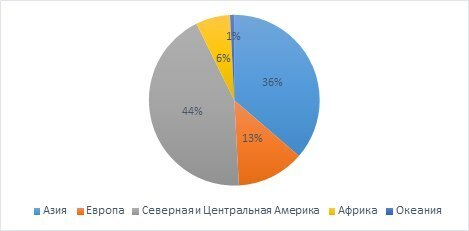
\includegraphics[width=0.6\textwidth]{assets/307-1}
	\caption*{\bfseries Рис. 1 - Поголовье лошадей по континентам}
\end{figure}

\begin{multicols}{2}

В развитии национальной экономики особую роль играют отрасли
промышленности. Отрасль промышленности является комплексом предприятий,
который имеют однотипное экономическое назначение производимой
продукции, общую техническую базу, особый профессиональный состав
работников, специфику работы, используют однородные потребляемые
материалы и характеризуются однотипностью технологических процессов.
Иными словами, отрасль промышленности объединяет предприя-тия, которые
производят однородную продукцию, используют похожие технологии и имеют
свой круг потребителей.

Анализ состояния перерабатывающей промышленности в рамках исследования
был проведен на примере мясной отрасли. Мясная промышленность -- отрасль
пищевой промышленности, перерабатывающая скот. По данным агентства
статистики Министерства национальной экономики Республики Казахстан по
состоянию на 1 июня 2023 года в Казахстане распределение численности
скота в Казахстане: овец -- 25, 9 млн голов (57\%); крупного рогатого
скота -- 10,5 млн голов (23\%); лошадей -- 4,5 млн голов (10\%); коз --
3,2 млн голов (7\%); верблюдов -- 292 тыс.голов (1\%) (Рисунок 2)
{[}2{]}.
\end{multicols}

\begin{figure}[H]
	\centering
	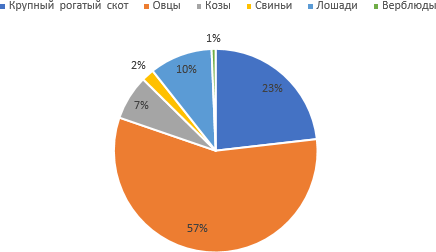
\includegraphics[width=0.6\textwidth]{assets/307}
	\caption*{Рис. 2 - Численность скота по состоянию на 1 июня 2023 г. в Казахстане}
\end{figure}

\begin{multicols}{2}


Современная экономика Казахстана ведет свой отсчет с 1991 года, когда
произошел распад СССР. С этого момента страна взяла курс на модернизацию
экономики, а также на интеграцию в экономическое пространство. В
Казахстане плановая рыночная модель экономики, которая в настоящее время
интенсивно развивается. Казахстан активно наращивает собственное
производство, прежде всего, развивая пищевую промышленность, в частности
мясную промышленность. Эта отрасль крайне важна, поскольку связана с
производством сырья, материалов и продуктов, направленных на
удовлетворение пищевых потребностей населения. Согласно динамике объема
рынка конины в Казахстане в период 1991-2022 гг.: наибольшая прибавка
поголовья лошадей в Казахстане наблюдается в 1999 г. -- 127,2 тыс.
голов, 2011 г. -- 121,5, 1992 г. -- 121,4 тыс.голов (Рисунок 3).
\end{multicols}

\begin{figure}[H]
	\centering
	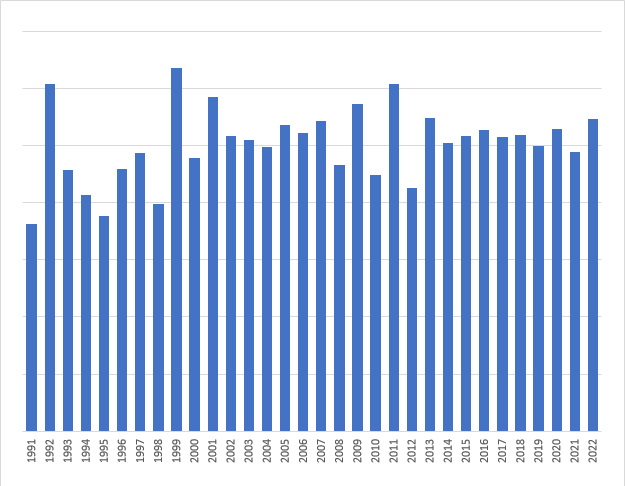
\includegraphics[width=0.6\textwidth]{assets/308}
	\caption*{Рис. 3 - Динамика объема рынка конины в Казахстане в 1991-2022 гг.,
	тыс.голов}
\end{figure}

\begin{multicols}{2}


Коневодство в Казахстане -- это важный вид деятельности в сельском
хозяйстве, которая в последнее время интенсивно развивается. Благодаря
особенным климатическим условиям, огромными запасами воды и большими
пастбищными хозяйствами, Акмолинская область является подходящей для
разведения лошадей. В 2023 году поголовье лошадей в областях составляло
4,5 млн голов, в том числе в сельскохозяйственных предприятиях 299 тыс.
голов (6,7 \%), у населения 1,9 млн голов (42,2 \%), в крестьянских
(фермерских) хозяйствах и у индивидуальных предпринимателей - 2,3 млн
голов (51,1 \%) {[}3{]}.

Казахстан входит в первую десятку стран мира с наиболее развитым
коневодством. В силу обширности территории, сложных дорожных условий,
многообразия природно-климатических зон и национальных традиций
использование лошадей в Казахстане остается многоплановым. Разводят
свыше 40 пород, по данным СтатБюро (2023), общее поголовье составляет
1,303 млн, из них около 30\% - продуктивные животные, около 4,5\% -
племенные и спортивные, остальные -- рабоче-пользовательные. Основное
пооголовье находится во владении акционерных обществ, кооперативов,
товариществ, фермерских и подсобных хозяйств. В структуре племенного
коневодства действуют около 100 конных заводов, около 300 племенных
ферм, государственные заводские конюшни и др. Всего насчитывается 1500
предприятий по разведению лошадей. Возрастают потребности в конине и
кумысе, расширяется ареал продуктивного коневодства. Стабильно
востребовано рабоче-пользовательное коневодство. Научно-обоснован-ная
потребность в поголовье лошадей всех направлений использования в
Казахстане -- свыше 6,2 млн голов {[}4{]}.
\end{multicols}

\begin{figure}[H]
	\centering
	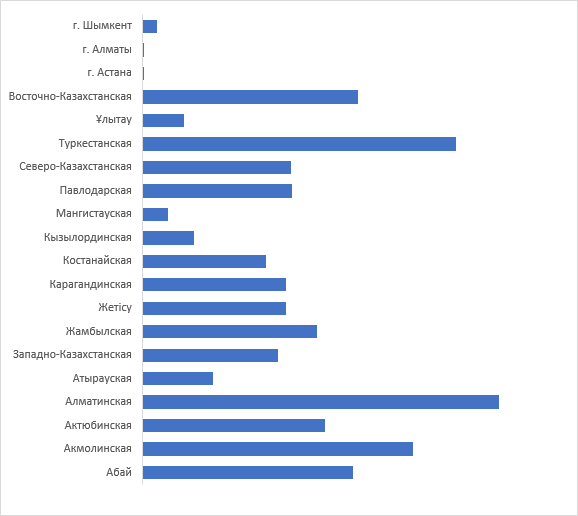
\includegraphics[width=0.8\textwidth]{assets/309}
	\caption*{Рис. 4 - Численность поголовья лошадей по состоянию на 1 июня по Республике Казахстан, голов
	}
\end{figure}

\begin{multicols}{2}

Наибольшая прибавка поголовья лошадей в Казахстане наблюдается в двух
регионах: Алматинская -- 221,5 тыс. голов; Туркестанская -- 194,8 тыс.
голов (Рисунок 4).

{\bfseries Материалы и методы.} ГОСТ 32225-2013 Лошади для убоя~Конина и
жеребятина в полутушах и четвертинах. Технические условия. Horses for
slaughter. Horseflesh in semi-carcasses and quarters. Specifications
{[}5{]}.

ГОСТ 27095-86 Конина и жеребятина в полутушах и четвертинах Технические
условия. Meat. Horse meat and young horse meat in half-carcasses and
quarters.~Specifications {[}6{]}.

Результаты и обсуждение. В продовольственной программе Казахстана
большое внимание уделяется развитию мясной промышленности. Поставлена
задача увеличить мясные ресурсы за счет развития скотоводства, в том
числе и коневодства.

Конина издавна имеет большое значение в питании населения Казахстана,
Кыргызстане, Якутии, Бурятии, Узбекистане, Татарстане, Башкортостане.
Она является одним из ценных видов мяса, так как более богата белками,
чем говядина и свинина.

Крупной базой коневодства является Казахстан. По численности поголовья
лошадей она занимает второе место среди бывших союзных республик. В
Казахстане продуктивное коневодство сложилось в самостоятельную отрасль
животноводства, перед которой поставлена задача -- удовлетворить
потребности населения в высококачественной конине. Здесь имеются
благоприятные условия для развития мясного коневодства.

Ароматное нежное мясо молодых лошадей считается ценным сырьем для
изготовления национальных изделий.

Резервы увеличения производства конины следующие: рост поголовья лошадей
в селах самостоятельной отрасли мясного коневодства, правильная
организация кормовой базы, кормление, нагулы, откорм и разведение
лошадей, сдаваемых на мясо, и х доращивание, борьба с потерями поголовья
скота, а также с потерями его упитанности при транспортировке на
предприятия.

Рост поголовья в коневодстве за последние пять лет составил 45,8\%, что
делает отрасль лидером в мясном и племенном животноводстве. Коневодство
по сравнению с другими направлениями животноводства ниже, а продукция
имеет устойчивый спрос и высокую маржинальную прибыль, поскольку
сбывается по цене выше говядины и баранины. Так, в ноябре 2023 г. цена
килограмма говядины в Казахстане составляла в среднем от 2,5 тыс. тенге
до 3,5 тыс. тенге в разных регионах страны, а баранины -- от 1,8 до 2,3
тыс. тенге. Конина же сбывалась в ценовом диапазоне от 1,8 до 3,5 тыс.
тенге за кг, и это при себестоимости в 400-500 тенге. Низкая
себестоимость производства конины обусловлена тем, что лошадей можно
пасти круглый год. Но при этом из-за более высоких вкусовых качеств и
традиций в Казахстане конина будет дороже и говядины, и баранины.

Согласно данным статистического бюро, потребление в Казахстане говядины
составило во втором квартале 2023 г. 5,6 кг на одного жителя страны, а
баранины -- 1,7 кг за тот же период. Это пока превышает потребление
конины - 1 кг.

При этом конина 2023 г. дорожала медленнее, чем два ее основных
конкурента по внутреннему рынку -- 13 \% рост в цене за 10 месяцев
против 15\% роста стоимости говядины за тот же период и 15,6\% роста
цены баранины {[}7{]}.

Популярность лошадиного мяса на рынке постепенно растет. Причиной тому
выступает состав продукта. Мясо является отличным источником белка. Как
объяснялось выше, эти белки выполняют определенные функции в живой
мышечной ткани и при преобразовании мышц в мясо. К ним относятся актин и
миозин (миофибриллярные белки), гликолитические ферменты и миоглобин
(саркоплазматические белки) и коллаген (белки соединительной ткани).
Поскольку белки, содержащиеся в мясе, обеспечивают рацион всеми девятью
незаменимыми аминокислотами, мясо считается полноценным источником
белка. Включает протеин -- не менее 15--20\%; воду -- 70\%; жиры в
количестве 2--5\%; золу -- около 1\%. Что касается микроэлементов, то в
составе конины основную часть занимают: калий, железо, натрий, фосфор и
др. Богата конина и на витамины. Такой состав предполагает высокую
энергетическую ценность продукта. По своей калорийности он относится к
числу среднекалорийных и составляет около 120-180 ккал на каждые 100 г
мяса. Диетологи утверждают, что конина рекомендована детям в качестве
первого прикорма, особенно страдающим аллергией {[}8{]}.

В рационе жиры, содержащиеся в мясе, служат переносчиками
жирорастворимых витаминов (А, D, Е и К) и поставляют необходимые
вещества не поставляемые организмом). Помимо своей роли запаса энергии,
жирные кислоты являются предшественниками в синтезе. Жирнокислотный
состав мяса зависит от нескольких факторов. Рацион питания лошадей при
откорме может существенно изменить состав жирных кислот мяса. Если
кормить добавками с высоким содержанием ненасыщенных жиров, жир, который
они откладывают в мышцах, будет иметь повышенный уровень ненасыщенных
жирных кислот. При классификации мяса мясо разделяется на разные классы
на основе ожидаемых пищевых качеств (например, внешнего вида, нежности,
сочности и вкуса) и ожидаемого выхода товарного мяса из тушки. В отличие
от процедур проверки мяса, системы классификации мяса значительно
различаются во всем мире. Эти различия во многом обусловлены тем, что в
разных странах действуют разные стандарты качества мяса. Например, в
Соединенные Штаты скот откармливают в первую очередь для производства
стейков и откармливают высококачественными зерновыми кормами для
достижения высокого количества по всей мускулатуре животного. Высокий
уровень качества мяса связан с более сочными, более ароматными и нежными
комбикормами при откорме {[}9{]}. Самым распространенным компонентом
мяса является -- вода. Однако, поскольку жировая ткань содержит мало
влаги или вообще не содержит ее, по мере увеличения процента жира в
куске мяса процент воды снижается. Таким образом, нежирная молодая
конина может содержать до 80 процентов воды, а полностью откормленная
конина --- до 50 процентов. Поскольку при приготовлении мяса теряется
вода, процентное содержание белка и жира в приготовленном мясе обычно
выше, чем в сыром.

На содержание миоглобина в скелетных мышцах влияет ряд факторов
кормления и процесса убоя. Мышцы представляют собой смесь двух разных
типов мышечных волокон: быстро сокращающихся и медленно сокращающихся,
пропорции которых различаются между мышцами. Быстро сокращающиеся
волокна имеют низкое содержание миоглобина, поэтому их еще называют
белые волокна. Медленно сокращающиеся волокна содержат большое
количество миоглобина и обладают большей способностью к окислительному
метаболизму. Эти волокна часто называют красные волокна. Следовательно,
темный цвет мяса является результатом относительно высокой концентрации
медленно сокращающихся волокон в мышцах животного. При составлении
перспективных планов содержания и откорма животных, на примере
производства конины, широко используются различные нормативы.
Применительно к табунному коневодству в экономической и
сельскохозяйственной литературе для отдельных регионов страны также
разрабатывались нормативные показатели рациона питания {[}10{]}.
Республика Казахстан с наличием огромных территорий естественных пастбищ
(180 млн га) имеет значительные перспективы в снабжении страны
экологически чистыми продуктами питания. Крупным резервом выполнения
Продовольственной программы республики является отгонное животноводство,
в частности, коневодство. Необходимо отметить, что на протяжении
последнего десятилетия государство приняло ряд программ, направленных на
развитие агропромышленного комплекса страны {[}11{]}.

Для обеспечения качества мясных продуктов из конины, необходимо
оптимизировать выход конечной продукции по всей цепочке создания
стоимости. Одним из факторов влияющих на повышение эффективности всей
цепочки создания стоимости является комплекс использования оборудования
для переработки. Начиная с конкретных процессов, таких как взвешивание,
нарезка и маркировка, до комплексных решений, таких как линии обвалки,
обрезки, приготовления мяса, нарезки на порции и формовки
мясопереработки с постоянным вниманием к гигиене и безопасности.
Количество оборудования будет зависеть от используемых процедур убоя и
переработки.

{\bfseries Выводы.} В настоящее время в Казахстане пищевая промышленность
развивается достаточно сбалансированно. Мясная отрасль нуждается в
разработке новых методов откорма с применением инновационных
информационно-технических решений и привлечении инвестиций для оснащения
высокопроизводительным оборудованием для переработки с целью обеспечения
повышения эффективности производства конины.

Повышение экономической эффективности позволит сделать коневодство одним
из рентабельных направлений животноводства, обеспечивающим необходимый
ресурс для устойчивого животноводства и удовлетворяющим растущий спрос
на белок в пище для быстро растущего населения.
\end{multicols}


\begin{center}
	{\bfseries Список литературы}
\end{center}

\begin{noparindent}

1. Продовольственная и сельскохозяйственная организация Объединенных
наций URL:\\http://www.fao.org/home/ru/ {[}Электронный ресурс{]}. (дата
обращения - 12.03.2024)

2. Данные Комитета по статистике Министерства национальной экономики
Республики Казахстан по состоянию на январь-октябрь 2023 года. -URL:
https://www.gov.kz/memleket/entities/economy?lang=ru {[}Электронный
ресурс{]}. (дата обращения 12.03.2024)

3. Бюро национальной статистики агентства по стратегическому
планированию и реформам \\Республики Казахстан по состоянию на 1 июня 2023
года. - URL: https://stat.gov.kz/ru/ {[}Электронный ресурс{]}. Дата
обращения - 12.03.2024

4. Большая Российская энциклопедия. - URL:
https://bigenc.ru/c/konevodstvo-394ab0 {[}Электронный ресурс{]}. Дата
обращения - 12.03.2024

5. ГОСТ 32225-2013. Лошади для убоя~Конина и жеребятина в полутушах и
четвертинах. Технические условия. Horses for slaughter. Horseflesh in
semi-carcasses and quarters. Specifications. -- Взамен ГОСТ 20079-74;
введ - 01.07.2015. --Москва: Межгосударственный стандарт. - М.: Изд-во
стандартов, 2015.

6. ГОСТ 27095-86. Конина и жеребятина в полутушах и четвертинах.
Технические условия. Meat. Horse meat and young horse meat in
half-carcasses and quarters.~
Specifications. - Взамен ГОСТ 20079-74; введ -- 01.01.1988. --Москва:
Межгосударственный стандарт. - М. : Изд-во стандартов, 2006.

7. Бас аграрлық сайт URL: https://eldala.kz {[}Электронный ресурс{]}.
(дата обращения - 12.03.2024)

8. Инербаева А.Т. Производители конины и ее переработка на качественные
мясные продукты.//\\Сибирский научно-исследовательский и технологический
институт переработки сельскохозяйствен-ной продукции Сибирского
Федерального научного центра агробиотехнологий Российской академии наук
(СибНИТИП СФНЦА РАН).- Материалы международной научно-практической конференции, посвященной 100-летию
доктора cельскохозяйственных наук, профессора, заслуженного деятеля
науки Российской Федерации и Республики Бурятия Мункоева Константина
Тармаевича. \\- Новосибирск, Россия. - 2019. -с.103-109

9. The American Association of Meat Processors (AAMP). --URL:
https://www.aamp.com/ \\(date of application - 03/12/2024)

10. Нурушева Г.М. Научное обоснование эффективности продуктивного
коневодства на Севере Казахстана // Известия Оренбургского
государственного аграрного университета, -2011. -№. 4(32-1). -С.
247-249.

11. Есенгалиева С.М., Мансурова М.А., Махмудов А.Д., Федорченко Л.В.
Современное состояние и тенденции развития животноводства в Республике
Казахстан.~~Economics: the strategy and practice. -2021. №16(2).
-P134-144. DOI 10.51176/1997-9967-2021-2-134-144.

\end{noparindent}

\begin{center}
{\bfseries References}
\end{center}

\begin{noparindent}

1. Prodovol\textquotesingle stvennaya i
sel\textquotesingle skokhozyaistvennaya organizatsiya Ob"edinennykh
natsii URL:\\ http://www.fao.org/home/ru/ {[}Elektronnyĭ resurs{]}. (data
obrashcheniya - 12.03.2024) {[}in Russian{]}

2. Dannye Komiteta po statistike Ministerstva
natsional\textquotesingle noĭ ekonomiki Respubliki Kazakhstan po
\\sostoyaniyu na yanvar\textquotesingle-oktyabr\textquotesingle{} 2023
goda. -URL: https://www.gov.kz/memleket/entities/economy?\\lang=ru
{[}Elektronnyĭ resurs{]}. (data obrashcheniya 12.03.2024) {[}in
Russian{]}

3. Byuro natsional\textquotesingle noi statistiki agentstva po
strategicheskomu planirovaniyu i reformam Respubliki\\ Kazakhstan po
sostoyaniyu na 1 iyunya 2023 goda. - URL: https://stat.gov.kz/ru/
{[}Elektronnyĭ resurs{]}. \\Data obrashcheniya - 12.03.2024 {[}in
Russian{]}

4. Bol\textquotesingle shaya Rossiiskaya entsiklopediya. - URL:
https://bigenc.ru/c/konevodstvo-394ab0 {[}Elektronnyĭ\\ resurs{]}. Data
obrashcheniya - 12.03.2024 {[}in Russian{]}

5. GOST 32225-2013. Loshadi dlya uboya Konina i zherebyatina v
polutushakh i chetvertinakh.\\ Tekhnicheskie usloviya. Horses for
slaughter. Horseflesh in semi-carcasses and quarters. Specifications. --
Vzamen GOST 20079-74; vved - 01.07.2015. --Moskva: Mezhgosudarstvennyi
standart. - M.: Izd-vo standartov, 2015. {[}in Russian{]}

6. GOST 27095-86. Konina i zherebyatina v polutushakh i chetvertinakh.
Tekhnicheskie usloviya. Meat. Horse meat and young horse meat in
half-carcasses and quarters.

Specifications. - Vzamen GOST 20079-74; vved -- 01.01.1988. --Moskva:
Mezhgosudarstvennyi standart. - M. : Izd-vo standartov, 2006. {[}in
Russian{]}

7. Bas agrarlyq sait URL: https://eldala.kz {[}Elektronnyĭ resurs{]}.
(data obrashcheniya - 12.03.2024) {[}in Russian{]}

8. Inerbaeva A.T. Proizvoditeli koniny i ee pererabotka na kachestvennye
myasnye produkty.//Sibirskii nauchno-issledovatel\textquotesingle skii i
tekhnologicheskii institut pererabotki
sel\textquotesingle skokhozyaistvennoi produktsii \\Sibirskogo
Federal\textquotesingle nogo nauchnogo tsentra agrobiotekhnologii
Rossiiskoi akademii nauk (SibNITIP\\ SFNTsA RAN), materialy mezhdunarodnoi
nauchno-prakticheskoi konferentsii, posvyashchennoi 100-letiyu doktora
cel\textquotesingle skokhozyaistvennykh nauk, professora, zasluzhennogo
deyatelya nauki Rossiiskoi \\Federatsii i Respubliki Buryatiya Munkoeva
Konstantina Tarmaevicha. - Novosibirsk, Rossiya. - 2019. -S.103-109
{[}in Russian{]}

9. The American Association of Meat Processors (AAMP). --URL:
https://www.aamp.com/ (date of \\application - 03/12/2024)

10. Nurusheva G.M. Nauchnoe obosnovanie effektivnosti produktivnogo
konevodstva na Severe \\Kazakhstana // Izvestiya Orenburgskogo
gosudarstvennogo agrarnogo universiteta, -2011. -№. 4(32-1). -S.
247-249. {[}in Russian{]}

11. Esengalieva S.M., Mansurova M.A., Makhmudov A.D., Fedorchenko L.V.
Sovremennoe sostoyanie i tendentsii razvitiya zhivotnovodstva v
Respublike Kazakhstan. Economics: the strategy and practice. -2021.
№16(2). -P134-144. DOI 10.51176/1997-9967-2021-2-134-144. {[}in
Russian{]}

\end{noparindent}

\emph{{\bfseries Сведения об авторах}}

\begin{noparindent}

Анель Т.К. - докторант НАО «Казахский агротехнический исследовательский
университет им. \\С.Сейфуллина», Астана, Казахстан, e-mail:
anel\_kostanova@mail.ru;

Шолпан Б.Б. - кандидат технических наук, и.о. ассоциированного
профессора НАО «Казахский агротехнический исследовательский университет
им. С.Сейфуллина», Астана, Казахстан, e-mail: \\baytukenova75@mail.ru;

Сауле Б.Б. - кандидат технических наук, и.о. ассоциированного профессора
АО «Казахский универси-тет технологии и бизнеса им. К. Кулажанова»,
Астана, Казахстан, e-mail: saule7272@mail.ru

\end{noparindent}

\emph{{\bfseries Information about authors}}

\begin{noparindent}

Anel T.K. - PhD student «S.Seifullin Kazakh Agrotechnical Research
University» NJSC, Astana, \\Kazakhstan, e-mail: anel\_kostanova@mail.ru;

Sholpan B.B. -- candidate of technical sciences, acting associate
professor «S.Seifullin Kazakh Agrotechnical Research University» NJSC,
Astana, Kazakhstan, e-mail: baytukenova75@mail.ru;

Saule B.B. -- candidate of technical sciences, acting associate
professor «Kazakh University of Technology and Business named after
K.Kulazhanov» JSC, Astana, Kazakhstan, e-mail: saule7272@mail.ru
\end{noparindent}
